%
% CMPT 473: Software Quality Assurance - A Course Overview
%
% Author: Jeffrey Leung
%

\documentclass[10pt, oneside, letterpaper, titlepage]{article}

\usepackage{amsmath}
\usepackage[ampersand]{easylist}
	\ListProperties(
		Progressive*=5ex,
		Space=5pt,
		Space*=5pt,
		Style1*=\textbullet\ \ ,
		Style2*=\begin{normalfont}\begin{bfseries}\textendash\end{bfseries}\end{normalfont} \ \ ,
		Style3*=\textasteriskcentered\ \ ,
		Style4*=\begin{normalfont}\begin{bfseries}\textperiodcentered\end{bfseries}\end{normalfont}\ \ ,
		Style5*=\textbullet\ \ ,
		Style6*=\begin{normalfont}\begin{bfseries}\textendash\end{bfseries}\end{normalfont}\ \ ,
		Style7*=\textasteriskcentered\ \ ,
		Style8*=\begin{normalfont}\begin{bfseries}\textperiodcentered\end{bfseries}\end{normalfont}\ \ ,
		Hide1=1,
		Hide2=2,
		Hide3=3,
		Hide4=4,
		Hide5=5,
		Hide6=6,
		Hide7=7,
		Hide8=8 )
\usepackage{geometry}
	\geometry{margin=1.2in}
\usepackage{graphicx}
	\graphicspath{ {img/} }
\usepackage[colorlinks=true, linkcolor=blue]{hyperref}
\usepackage{lmodern} % Allows the use of symbols in font size 10; http://ctan.org/pkg/lm
\usepackage{textcomp} % Allows the use of \textbullet with the font
\usepackage{verbatim}

\renewcommand{\arraystretch}{1.2}
\renewcommand{\familydefault}{\sfdefault}

\title{CMPT 473: Software Quality Assurance \\\medskip \Large A Course Overview}
\author{Jeffrey Leung \\ Simon Fraser University}
\date{Spring 2020}

\begin{document}

	\maketitle
	\tableofcontents
	\clearpage

	%
% CMPT 213: Object Oriented Design in Java - A Course Overview
% Section: Introduction
%
% Author: Jeffrey Leung
%

\section{Introduction}
	\label{sec:introduction}
\begin{easylist}

& Standards:
	&& Make fields private when possible

& Commenting:
	&& Comment purpose of a class
	&& Name fields/methods/parameters so comments are unnecessary

& When possible, convert strings to non-string types internally for consistency

& \textbf{Clean code:} Code which is correct, easy to read/maintain, and conforms to a standard

& Software design:
	&& 4 steps:
		&&& Requirements
		&&& Design and implementation
		&&& Verification
		&&& Evolution
	&& Designing involves identifying classes, responsibilities, and relationships to create a diagram
	&& Implementation process options:
		&&& \textbf{Skeleton code:} Beginning minimal parts/features of a system
		&&& \textbf{Component-wise:} Creating components one at a time
	&& Methods of integrating code from multiple people:
		&&& \textbf{Continual integration:} Gradual system growth by constantly integrating changes
		&&& \textbf{Big Bang integration:} Building all parts separately without integrating until the end

& \textbf{Feature envy:} Characteristic of a class which relies heavily on another class
& Warning sign: Characteristic of a method which operates more strongly on another object than its own
& \textbf{Deprecation:} State where a public interface is no longer supported or recommended, and is slated to be removed in the future


& \textbf{try-catch:} Structure which watches for an exception and handles it
	&& Only one exception can be live at a given time
	&& \textbf{finally clause:} Optional clause after catch clauses which is executed regardless of the result
		&&& If exception is thrown, the finally clause is executed immediately afterwards
	&& \textbf{try-with-resources:} Block which cleans up a resource when a try block exits

& Exception: Issue which may be fixable and is not out of the software's control
	&& \textbf{Checked exception:} Exception which must be caught or listed in a throws clause
	&& \textbf{Unchecked exception:} Exception which will automatically propagate and does not require catching
		&&& E.g. RuntimeException
		&&& Preferred as it does not require modification of methods between try/catch, which decouples code

\end{easylist}
\clearpage
	

	%
% CMPT 473: Software Quality Assurance - A Course Overview
% Section: Debugging
%
% Author: Jeffrey Leung
%

\section{Debugging}
	\label{sec:debugging}
\begin{easylist}

& \textbf{Debugging:} Application of the scientific method to find and eliminate an incorrect behaviour

& Steps:
	&& Ignore assumptions
		&&& Mental model of software may be incorrect
		&&& Comments may be incorrect
	&& Reproduce the behaviour
	&& Brainstorm possible reasons why the incorrect behaviour occurred
	&& Choose the most testable and likely hypotheses

& Debugging framework features:
	&& Breakpoints (conditional)
	&& Stepping through/over code
	&& State:
		&&& Print/display
		&&& Modification
		&&& Watchpoints
	&& Call functions

\end{easylist}
\subsection{Bug Reporting}
	\label{subsec:bug-reporting}
\begin{easylist}

& Perspectives:
	&& Developer: How a bug should be handled
	&& Client/teammate: How a bug should be reported/fixed

& Error messages should contain:
	&& What is incorrect
	&& Where the error occurred
	&& When the error occurred

& Good error messages allow you to:
	&& Reproduce a failure
	&& Find the original creator
	&& Combine duplicate error reports
	&& Identify causes
	&& Prioritize
	&& Identify workarounds
	&& Create an accurate fix

& Prioritize bugs by:
	&& Frequency
	&& Risk level or consequence
	&& Recency of introduction

& Bug reports should contain:
	&& Summary
	&& What happened, when, where
	&& Expected result
	&& Steps to reproduce
	&& Product, version, feature
	&& Platform and environment
	&& Severity/priority
	&& Owner(s)
	&& Duplicate(s)

\end{easylist}
\clearpage
	
	%
% CMPT 473: Software Quality Assurance - A Course Overview
% Section: Types of Testing
%
% Author: Jeffrey Leung
%

\section{Types of Testing}
	\label{sec:types-of-testing}
\begin{easylist}

& Test cases:
	&& Require an input and expected output/state/behaviour
	&& \textbf{Oracle:} Evaluation of the output/behaviour of a test
	&& \textbf{Mock:} Entity which is used to measure or examine behaviour
	&& \textbf{Stub:} Fake entity which is used during testing to replace a component

& If external state is uncontrolled, tests will be nondeterministic
	&& Factors causing lack of control:
		&&& Lack of isolation
		&&& Asynchronous behavior
		&&& Remote services
		&&& Time
		&&& Resource leaks

& \textbf{Coverage/adequacy:} Measurement of how well a test suite addresses quality criteria

& \textbf{Test Driven Development (TDD)}: Software testing where unit tests are created first and used to drive development

& \textbf{Unit testing}: Software testing of the smallest possible components
	&& Principles include component isolation, simplicity, ease of understanding

& \textbf{Integration testing}: Software testing based on the connection of multiple components

& \textbf{Acceptance testing}: Software testing based on acceptance criteria

& \textbf{Black-box testing:} Software testing based on the external input specification of a system
	&& Involves \hyperref[sec:input-space-partitioning]{input space partitioning}
& \textbf{White-box testing:} Software testing based on the internal program structure of a system
	&& Involves \hyperref[sec:graph-coverage]{graph coverage}

& \textbf{Fuzz testing:} Method of exploratory software testing which inputs randomly mutated data into a program to evaluate random inputs

& Test scenarios can be concrete (e.g. $x = 5$) or abstract (e.g. for all $x$, $x > 0$)
	&& Abstract test cases can generate a test and check the oracle, using:
		&&& Testing with randomly generated values
		&&& Symbolic execution

& Testing strategies which evaluate the existing test suite for effectiveness:
	&& MC/DC
	&& Mutation testing

\end{easylist}
\clearpage

	%
% CMPT 473: Software Quality Assurance - A Course Overview
% Section: Property-Based Testing
%
% Author: Jeffrey Leung
%

\section{Property-Based Testing}
	\label{sec:property-based-testing}
\begin{easylist}


& \textbf{Property-based testing:} Testing which generates tests to evaluate functional properties/requirements
	&& Mathematical representation of an expectation

& Common test strategies:
	&& \textbf{Symmetry:} Test strategy where operations are performed to return to the original value
	&& \textbf{Alternative:} Test strategy where a value is compared with a value generated from alternative solutions
	&& \textbf{Induction:} Test strategy
	&& \textbf{Idempotence:} Test strategy where performing an operation more than once has no effect
	&& \textbf{Invariant:} Test strategy where a property of a preprocessed value must be equal to the property of a processed value

\end{easylist}
\clearpage

	%
% CMPT 473: Software Quality Assurance - A Course Overview
% Section: A/B Testing
%
% Author: Jeffrey Leung
%

\section{A/B Testing}
	\label{sec:a-b-testing}
\begin{easylist}

& \textbf{A/B testing:} Hypothesis testing which provides different services to randomly selected individuals
	&& Requires a hypothesis and population to test

& Used to evaluate:
	&& Usability improvements
	&& Perforamnce improvements
	&& Promotion effectiveness
	&& Gradual rollouts

& Possible issues:
	&& Uncontrolled influencing factors
	&& Populations may not be representative
	&& False positives/negatives
		&&& \textbf{p-hacking:} Altering results by executing many tests to compound the effect of false positives/negatives, and choosing exactly when to stop based on the results
		&&& \textbf{Regression to the mean:} Tendency for results to return to relatively normal levels after an extreme event
			&&&& E.g. Poorly performing students are placed in a program, after which their grades improve

& Ways to mitigate issues:
	&& Calculate significance and test amount beforehand, rather than stopping when significance is reached

\end{easylist}
\subsection{Hypothesis Testing}
	\label{subsec:hypothesis-testing}
\begin{easylist}

& T-Test: Comparison between samples of populations
	&& Modeled as a distribution
	&& Requires the data to have a known variance, independence from other factors

& Sequential testing may have bounding criteria for when to stop early

& \textbf{Multi-armed bandit:} Testing technique which determines the best of multiple options based on evidence so far
	&& Requirements:
		&&& Reward probabilities do not change
		&&& Sampling is singular, instantaneous, and independent
		
	&& \textbf{$\epsilon$-greedy strategy:} Multi-armed bandit technique where the greater the previous sample proportion, the more likely the population is sampled
		&&& Sensitive to variance
		
	&& \textbf{Thompson sampling:} Multi-armed bandit technique where the probability of the best arm is chosen
		
\end{easylist}
\clearpage


	%
% CMPT 473: Software Quality Assurance - A Course Overview
% Section: Input Space Partitioning
%
% Author: Jeffrey Leung
%

\section{Input Space Partitioning}
	\label{sec:input-space-partitioning}
\begin{easylist}

& \textbf{Input Space Partitioning:} Division of potential inputs into classes where each input in a class should yield identical output

& \textbf{Input Domain Model:} Description of possible test inputs through discrete partitions which are disjoint and cover the entire domain
	&& \textbf{Interface-based approach:} Choosing inputs for a domain model based on parameters and domains
	&& \textbf{Functionality/requirements-based approach:} Choosing inputs for a domain model based on behaviours or functionality in the specification

& Process:
	&& Identify and isolate the component under test
	&& Identify inputs
		&&& Possible values to be partitioned:
			&&& Parameters and inputs
			&&&& Object state
			&&&& Global state
			&&&& File contents
	&& Identify characteristics of each input to divide into possible values
	&& Identify constraints
		&&& Characteristics to consider:
			&&&& Preconditions and postconditions
			&&&& Relationships to special values
			&&&& Relationships between variables
	&& Select representative values from an input block, including:
			&&&& Expected/valid values
			&&&& Special values
			&&&& Invalid values
			&&&& Boundary values

& E.g. Given a command to FIND instances of a PATTERN in a FILE:
	&& The component is the FIND command
	&& The parameters are the pattern to search for, the filename, and the file contents
	&& The characteristics include:
	 	&&& Is the pattern empty?
		&&& Is the length of the pattern contents less than, the same as, or greater than the length of the longest line in the file?
		&&& Does the pattern have quotation marks enclosing it?
		&&& Are ther escaped quotation marks in the pattern?
		&&& Is the filename empty?
		&&& Does the file exist?
		&&& Is the file a directory?
		&&& Is the file blank?
		&&& Does the file have a blank line?
		&&& Is there a line in the file matching the pattern multiple times?

\end{easylist}
\subsection{Test Combination Strategies}
	\label{subsec:input-space-partitioning:test-combination-strategies}
\begin{easylist}

& * means any value is valid

& \textbf{Each Choice:} From each block, use at least one value in at least one test
	&& Size: Largest domain
	&& Does not cover many possible conflicting states
	&& E.g. Given inputs A/B/C and 1/2, an adequate set of tests are:
		&&& A 1
		&&& B 2
		&&& C *

& \textbf{Pair Wise:} From each block, choose 1 value and test it at least once with every value from every other block
	&& Size (lower bound): $\geq$ the product of the domain sizes of the two largest partitions
	&& E.g. Given inputs A/B/C, 1/2, and X/Y, an adequate set of tests are:
		&&& A 1 X
		&&& A 2 Y
		&&& B 1 Y
		&&& B 2 X
		&&& C 1 *
		&&& C 2 *

& \textbf{T-Wise:} From each block, test 1 value for each group of $T$ characteristics
	&& Size: $\geq$ product of the $T$ largest domain partitionings

& \textbf{Base Choice:} Create a base test and create tests by changing only a single value and fixing the others
	&& Size: 1 base test plus one for each other unselected block
	&& Base case must be a valid positive test

& Hierarchy of test type satisfaction:
	&& All combinations includes all T-Wise tests and Multiple Base Choice testing
		&&& T-Wise testing includes all Pair-Wise tests
			&&&& Pair-Wise tests includes all Each Choice tests
		&&& Multiple Base Choice testing includes all Base Choice tests
			&&&& Base Choice tests includes all Each Choice tests

\end{easylist}
\clearpage


	%
% CMPT 473: Software Quality Assurance - A Course Overview
% Section: Graph Coverage
%
% Author: Jeffrey Leung
%

\section{Graph Coverage}
	\label{sec:graph-coverage}
\begin{easylist}

& \textbf{Control flow graph (CFG):} Graph where nodes represent code and edges represent paths taken
	&& Types of nodes: Entry, decision/branch, join, exit
	&& For a while loop, see figure~\ref{img:flow-diagram-while}
	&& For a for loop, see figure~\ref{img:flow-diagram-for}
	&& For a switch statement, see figure~\ref{img:flow-diagram-switch}
	&& For a short-circuited if statement, see figure~\ref{img:flow-diagram-if-shortcircuit}

\end{easylist}

\begin{figure}[!htb]
	\centering
	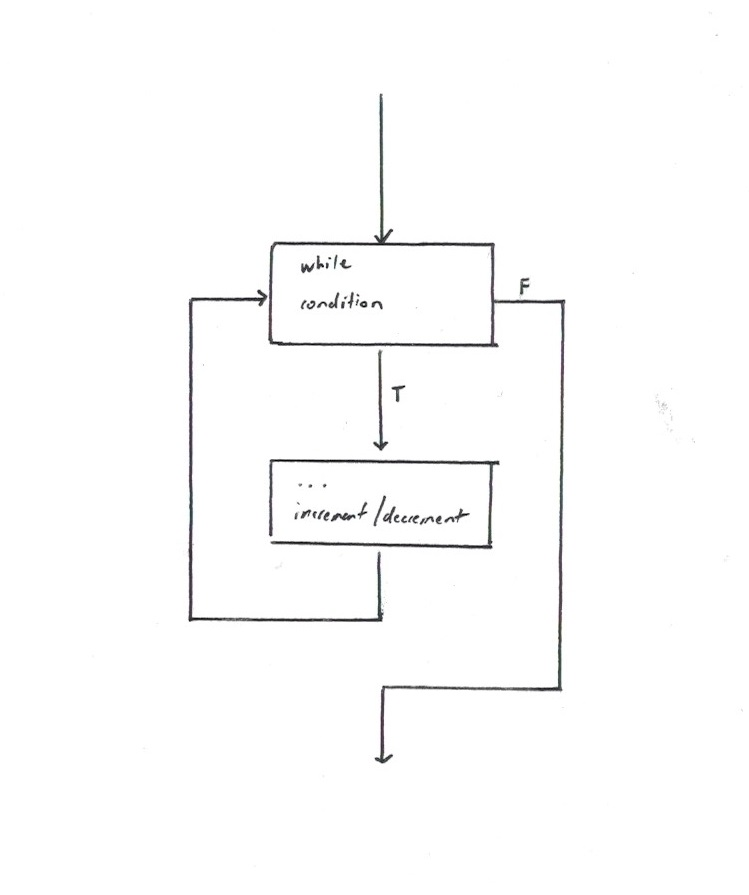
\includegraphics[width=.5\linewidth]{flow-diagram-while}
	\caption{Control Flow Graph of a while loop}
	\label{img:flow-diagram-while}
\end{figure}

\begin{figure}[!htb]
	\centering
	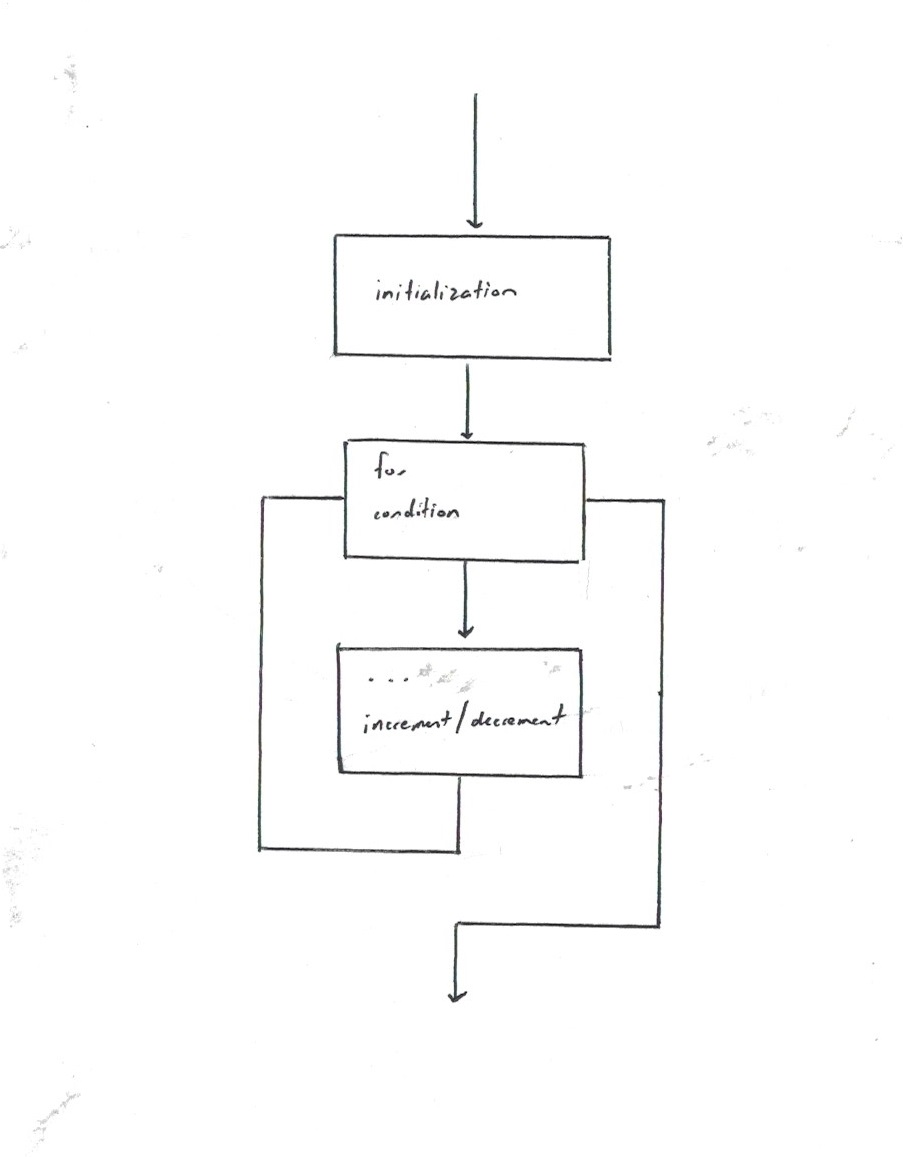
\includegraphics[width=.5\linewidth]{flow-diagram-for}
	\caption{Control Flow Graph of a for loop}
	\label{img:flow-diagram-for}
\end{figure}

\begin{figure}[!htb]
	\centering
	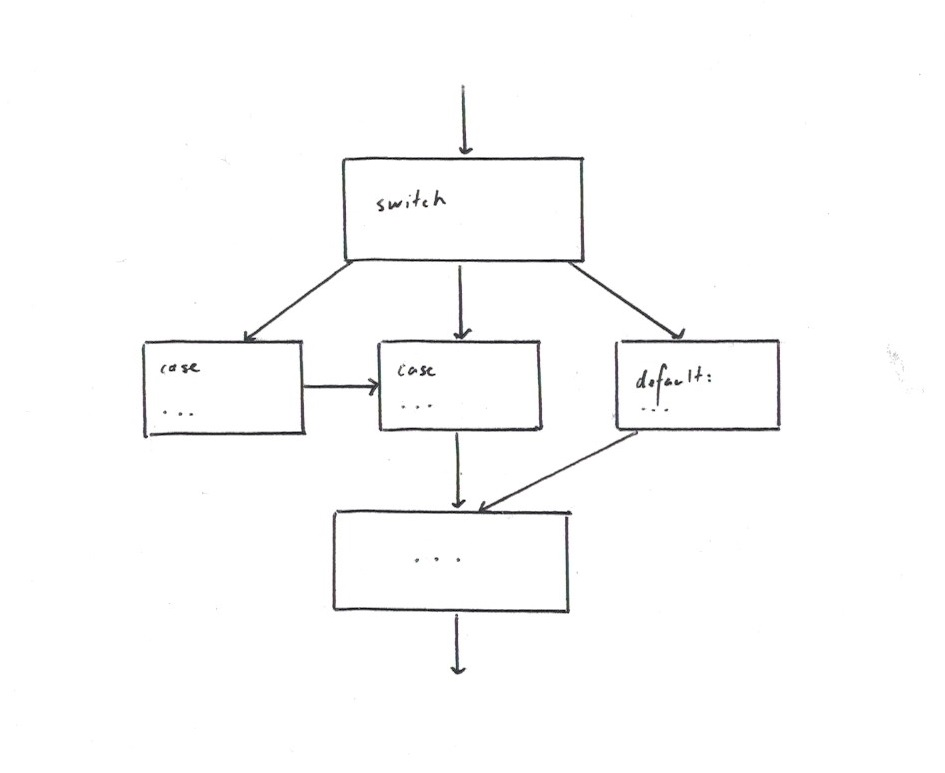
\includegraphics[width=.5\linewidth]{flow-diagram-switch}
	\caption{Control Flow Graph of a switch statement}
	\label{img:flow-diagram-switch}
\end{figure}

\begin{figure}[!htb]
	\centering
	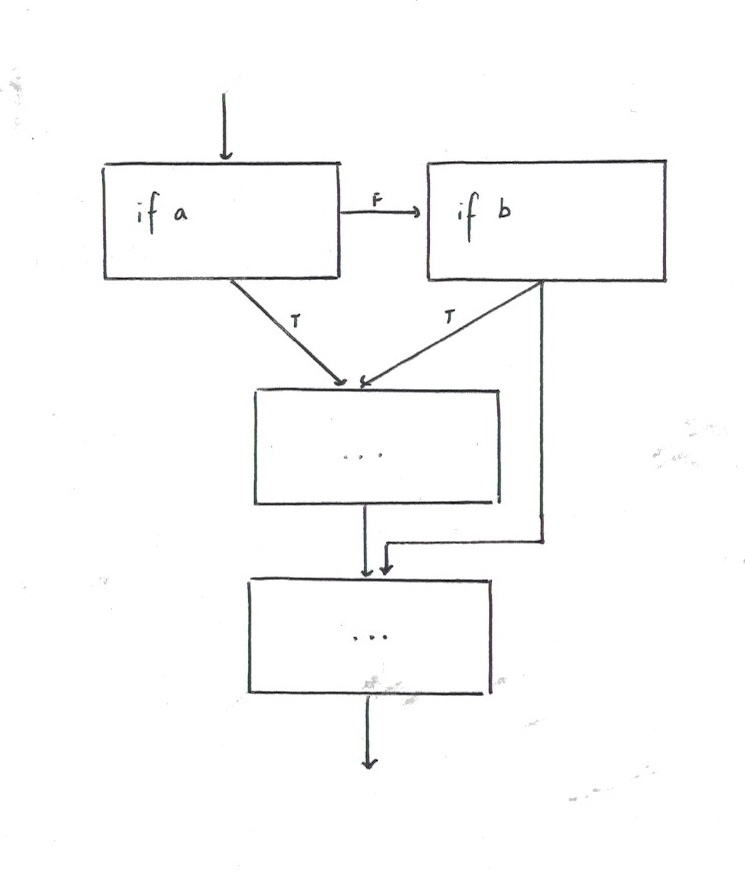
\includegraphics[width=.5\linewidth]{flow-diagram-if-shortcircuit}
	\caption{Control Flow Graph of a if statement short-circuited}
	\label{img:flow-diagram-if-shortcircuit}
\end{figure}

\begin{easylist}

& Edge coverage (i.e. all branches used) is a superset of node coverage

& \textbf{Complete path coverage:} Coverage of all possible paths through the graph
	&& Reason: Permutations/combinations of multiple possible paths can affect results
	&& Infeasible/intractible because it would entail combinatorial explosion and inability to efficiently test looping paths

& \textbf{Edge pair coverage:} Coverage which includes every path of length $<= 2$
& \textbf{Specified path coverage:} Coverage which tests $k$ paths for a given $k$

& \textbf{Reachability}: Property of a piece of code which may or may not be executable based on states
	&& \textbf{Syntactic reachability:} Analysis of reachability based on the structure of the code
	&& \textbf{Semantic reachability:} Analysis of reachability based on the meaning of the code (cannot be checked by an automated program)

& Testing loops is relevant when each iteration may affect the next
	&& \textbf{Simple path:} Acyclic path between nodes where no node appears more than once (except first/last)
	&& \textbf{Prime path:} Simple path which is not a subpath of any other simple path
		&&& I.e. A simple path which cannot be extended
		&&& E.g. Simple path which starts and ends at the same node
	&& \textbf{Tour:} Path which is a subpath of another
		&&& Mathematical definition: A path $p$ tours path $q$ if $q$ is a subpath of $p$
		&&& Tour with sidetrips: Tour where every edge of the superpath appears in the same order in the subpath
		&&& Tour with detours: Tour where every node of the superpath appears in the same order in the subpath

& \textbf{def-use pair:} Definition statement and the next relevant uses of the variable (before reassignment)
	&& Used to test along data flow
	&& Possible test approaches:
		&&& All defs coverage: Every def must be covered by at least one test of its uses
		&&& All uses coverage: Every use must be tested with least one definition
		&&& All def-use pairs coverage
		&&& All def-use paths coverage: All simple paths between def-use pairs are covered

& Path/branch coverage is insufficient due to scalability and complex conditions (e.g. non-short-circuiting) which do not have the notion of a path

\end{easylist}
\clearpage

	%
% CMPT 473: Software Quality Assurance - A Course Overview
% Section: Logic-Based Coverage
%
% Author: Jeffrey Leung
%

\section{Logic-Based Coverage}
	\label{sec:logic-based-coverage}
\begin{easylist}

& \textbf{Predicate coverage:} Each boolean expression must be tested as true and false in at least one test each
& \textbf{Clause coverage:} Each clause must be tested as true and false in at least one test
& \textbf{Combinatorial/Multiple Condition coverage:} Each possible combination of clauses must be tested

& Clause determines the outcome of a predicate if changing only the value of that clause changes the outcome of the predicate

& \textbf{Modified Condition/Decision Coverage (MCDC):} Coverage demonstrating that each entry/exit is used, each decision can take every possible outcome, each clause can take every possible outcome, and each clause independently can impact the outcome
	&& Based on the behaviour how one clause affects the entire expression
	&& Ensures that each clause has an impact
	&& Not effective to generate a test suite as the drive to create minimal tests interferes with MC/DC
	&& Used to check test suites generated using other strategies

& Determining the impact of a predicate
	&& Process for a given predicate $a$:
		&&& Create two clauses, one which replaces $a$ with $\#T$ (true) and the other which replaces $a$ with $\#F$ (false)
		&&& Set these two clauses as not equal to each other
		&&& Solve the equation
		&&& If the equation is not equal, then the predicate has impact
		
	&& Example: Given $(a \land b) \lor (a \land \neg b)$, prove whether $a$ has impact or not.
		&&& Let $a = T$ for one version of the clause, and $a = F$ for another version of the clause.

		\end{easylist}
		\begin{align*}
		(T \land b) \lor (T \land \neg b)
		& \stackrel{?}{=} (F \land b) \lor (F \land \neg b) \\
		b \lor \neg b
		& \stackrel{?}{=} F \lor F \\
		T
		& \stackrel{?}{=} F
		\end{align*}
		\begin{easylist}
		
		&&& The expression evalutes to $T \neq F$. Therefore $a$ has impact.

& Process of creating a minimal test suite using MC/DC:
	&& Change all compared expressions into clauses, each represented by one predicate
	&& Create a minimal set of logical assignments where, for each predicate, there are at least two assignments where:
		&&& The values of the predicate and result both differ, and
		&&& The values of all other predicates match
	&& Create a test suite with the original inputs set to specific values to satisfy the predicate values

	&& Example: Given $a \lor (b \land c)$, generate a minimal set of tests to demonstrate MCDC coverage.
		&&& See figure~\ref{fig:mcdc-example-1}.
		&&& Test entries 1 and 2 show the impact of $a$.
		&&& Test entries 2 and 3 show the impact of $b$.
		&&& Test entries 3 and 4 show the impact of $c$.
		
		\end{easylist}
		\begin{figure}[!htb]
			\centering
			\begin{tabular}{ c c c | c }
				a & b & c & Result \\
				\hline
				T & F & T & T \\
				F & F & T & F \\
				F & T & T & T \\
				F & T & F & F
			\end{tabular}
			\caption{MCDC Example Test Suite}
			\label{fig:mcdc-example-1}
		\end{figure}
		\begin{easylist}

	&& Example: Given $(a \land b \land c) \lor (d \land a)$, generate a minimal set of tests to demonstrate MCDC coverage.
		&&& See figure~\ref{fig:mcdc-example-2}.
		&&& Test entries 1 and 2 show the impact of $a$.
		&&& Test entries 2 and 3 show the impact of $d$.
		&&& Test entries 3 and 4 show the impact of $c$.
		&&& Test entries 4 and 5 show the impact of $b$.
		
		\end{easylist}
		\begin{figure}[!htb]
			\centering
			\begin{tabular}{ c c c c | c }
				a & b & c & d & Result \\
				\hline
				F & T & F & T & F \\
				T & T & F & T & T \\
				T & T & F & F & F \\
				T & T & T & F & T \\
				T & F & T & F & F
			\end{tabular}
			\caption{MCDC Example Test Suite}
			\label{fig:mcdc-example-2}
		\end{figure}
		\begin{easylist}

\end{easylist}
\clearpage

	%
% CMPT 473: Software Quality Assurance - A Course Overview
% Section: Mutation Analysis and Testing
%
% Author: Jeffrey Leung
%

\section{Mutation Analysis and Testing}
	\label{sec:mutation-analysis-and-testing}

\subsection{Mutant Fundamentals}
	\label{subsec:mutation-analysis-and-testing:mutant-fundamentals}
\begin{easylist}

& \textbf{Mutant:} Valid program which behaves differently from the original
	&& Involves smallest possible changes
	&& Invalid (and not counted in the mutation score) if:
		&&& Not compilable (still born)
		&&& Killed by most test cases (trivial)
		&&& Equivalent to the original program or to other mutants (redundant; can be undecidable)
	&& A valid mutant must satisfy the reachability, infection, and propagation model:
		&&& \textbf{Reachability:} Ability of the fault to be executed by a test
		&&& \textbf{Infection:} Ability of a fault to cause the program state to differ
		&&& \textbf{Propagation:} Ability of the differing program state to affect the output

& \textbf{Mutation operator:} Systematic change applied to produce a mutant
	&& \textbf{Intraprocedural mutations:} Modifying the internal values or operators of a procedure
		&&& E.g. (Optionally negated) absolute value insertion, arithmetic/relational/conditional operator replacement
	&& \textbf{Interprocedural mutations:} Modifying the inputs of a procedure
		&&& E.g. Parameter values, call target, incoming dependencies

& \textbf{Kill:} Characteristic of a test which produces a different outcome on a mutant than the original program
	&& Formal definition: A test $t$ kills a mutant $m$ if $t$ produces a different outcome on $m$ than the original program
	&& \textbf{Weakly kill:} A mutant test which results in different internal state
		&&& Satisfies reachability and infection, but not propagation
	&& \textbf{Strongly kill:} A mutant test which results in different output
		&&& Satisfies reachability, infection, and propagation

& Difficulties:
	&& Managing and executing a large amount of mutants
	&& Identifying identical mutants

\end{easylist}
\subsection{Fault Seeding}
	\label{subsec:mutation-analysis-and-testing:fault-seeding}
\begin{easylist}

& \textbf{Fault seeding:} Inserting expected faults to be killed
	&& Equation: $$\frac{\textrm{\# of mutants which killed a bug}}{\textrm{\# of mutants}}$$
	&& Issues:
		&&& Faults may not be meaningful
		&&& May forget to remove the faults

\end{easylist}
\subsection{Mutation Testing}
	\label{subsec:mutation-analysis-and-testing:mutantion-testing}
\begin{easylist}

& \textbf{Mutation analysis:} Ability to find bugs using a mutant
& \textbf{Mutation testing:} Process of creating a test suite which covers a representative set of mutants
	&& Given an unkilled mutant, improve the test suite by adding a test which kills it
	&& \textbf{Representative set:} Set of mutants which covers all possible faults

& \textbf{Mutation score:} Quantitative score of mutation analysis effectiveness
	&& Invalid mutants are not counted
	&& Equation: $$\frac
			{\textrm{\# of non-duplicated mutants which kill a bug}}
			{\textrm{\# of non-equivalent, non-duplicated mutants}}
			$$

& Manage scalability by:
	&& Filter based on coverage
	&& Short circuit tests
	&& Testing multiple mutants simultaneously

& Test coverage:
	&& \textbf{Weak mutation coverage}: For each mutant, the test suite contains a test which weakly kills the mutant
	&& \textbf{Strong mutation coverage}: For each mutant, the test suite contains a test which strongly kills the mutant

\end{easylist}
\clearpage

	%
% CMPT 473: Software Quality Assurance - A Course Overview
% Section: Regression Testing
%
% Author: Jeffrey Leung
%

\section{Regression Testing}
	\label{sec:regression-testing}
\begin{easylist}

& \textbf{Regression testing:} Method of testing which ensures previous functionality is preserved, supporting change

& Unexpected behaviour can be caused by:
	&& New environments
	&& Modifying other components

& Regression test suite is a subset of the test suite

& Components are tests for:
	&& Previously fixed bugs
	&& Units
	&& System

& Upon a failing test, one or more of the following should occur:
	&& Fix the software bug
	&& Fix stale test inputs
	&& Change expected behaviour

\end{easylist}
\subsection{Managing Test Suite Size}
	\label{subsec:regression-testing:managing-test-suite-size}
\begin{easylist}

& Limit regression test suite size by preventing redundant tests (e.g. not useful behaviour, not covered by adequacy criteria)

& Choosing a subset of tests:
	&& Conservative approach: Run all tests
	&& Cheap approach: Run tests which have requirements relating to the modified lines
	&& Middle ground approach: Run tests affected by how changes propagate by software
		&&& \textbf{Change impact analysis:} Identification of how a change affects other components

\end{easylist}
\clearpage


	%
% CMPT 473: Software Quality Assurance - A Course Overview
% Section: Program Analysis
%
% Author: Jeffrey Leung
%

\section{Program Analysis}
	\label{sec:program-analysis}
\begin{easylist}

& \textbf{Program analysis:} Tools and techniques which automatically analyze software behaviour

& \textbf{Dynamic analysis:} Analysis about a single instance of program execution
	&& Can be computationally expensive
	&& Does not examine all possible executions

& \textbf{Static analysis:} Analysis on source code about all possible executions
	&& Undecidability prevents some analyses
	&& \textbf{Abstract interpretation:} Static analysis method which simulates different execution paths

& False positives/negatives may occur

& Examples:
	&& Valgrind: Dynamic binary instrumentation tool to check for memory leaks
		&&& Only works on executables which provide both stack and heap allocated memory
	&& Clang sanitizers: Compile-time instrumentation tools to analyze safety of usage

\end{easylist}
\clearpage

	%
% CMPT 473: Software Quality Assurance - A Course Overview
% Section: Test Planning
%
% Author: Jeffrey Leung
%

\section{Test Planning}
	\label{sec:test-planning}
\begin{easylist}

& \textbf{Test plan:} Documentation of testing goals, concerns, methodology, metrics
	&& Guides testing process

& \textbf{Attribute-component-capability (ACC) testing:} Analysis of how testing addresses user-focused importance of components
	&& Test requirements and case count are sorted into their corresponding cell
	&& \textbf{Attribute:} High-level nonfunctional property to ensure (e.g. fast, secure)
	&& Component: Entity or grouping of software
	&& \textbf{Capability:} A characteristic of the system which supports a component having a particular attribute (e.g. for a database being secure, passwords should not be stored in plaintext)

\end{easylist}
\clearpage


	%
% CMPT 473: Software Quality Assurance - A Course Overview
% Section: Automated Test Generation
%
% Author: Jeffrey Leung
%

\section{Automated Test Generation}
	\label{sec:automated-test-generation}
\begin{easylist}

& \textbf{Automated test generation:} Executing program analysis to automatically derive tests

& \textbf{Fuzz testing:} Automated test generation method which creates sample program inputs
	&& \textbf{Generational (model-based) fuzz testing:} Fuzz testing method which creates inputs based on a predefined model
		&&& Inputs will be valid; cannot test invalid inputs
	&& \textbf{Mutational (heuristic change based) fuzz testing:} Fuzz testing method which creates inputs based modifying a test suite
		&&& Given a corpus of inputs, evolve new inputs; if the input tests a new area of the program, add it to the corpus
			&&&& Criteria can be different lines of code, more/less memory, etc.
		&&& Inputs may not necessarily be valid

& \textbf{Symbolic execution:}  Automated test generation method which replaces program inputs with symbolic values and calculates inputs based on constraints
	&& \textbf{Concolic (dynamic symbolic) traversal:} Symbolic execution where values are maintained as symbolic, then calculated at the end to reveal every possible path

& \textbf{Execution generated testing:} Symbolic execution where some values are set to be concrete

& \textbf{Execution tree:} Graph of the possible paths taken by a program

\end{easylist}
\clearpage


	%
% CMPT 473: Software Quality Assurance - A Course Overview
% Section: Performance
%
% Author: Jeffrey Leung
%

\section{Performance}
	\label{sec:performance}
\begin{easylist}

& Performance areas include:
	&& Speed/runtime
	&& Resource management
	&& Throughput
	&& Responsiveness
	
& Analyzed differently depending on component granularity (e.g. system-level, instruction-level)

& Strategies of measuring performance:
	&& Identify area of interest

& Evaluating results:
	&& Be aware of:
		&&& Warm-up time
		&&& Caching
	&& Measure and compare across changes
	&& Run many executions and take the average
	
& Measurement of results:

	&& \textbf{Arithmetic mean:} Average of measurements which measure the same value
		&&& Equation:
\begin{equation}
\frac{ \displaystyle \sum_{i=1}^N r_i }{N}
\end{equation}

	&& \textbf{Harmonic mean:} Average of measurements which report rates (e.g. throughput for multiple tasks)
		&&& Represents the constant rate required for the same amount of time
		&&& Calculated by dividing the total number of rates by the rate per unit (inversion of the rate)
		&&& Equation:
\begin{equation}
\frac{N}{ \displaystyle \sum_{i=1}^N \frac{1}{r_i} }
\end{equation}
	&& \textbf{Geometric mean:} Average of measurements which represent different values
		&&& A change in any benchmark affects the final value proportionally
		&&& Represents a multiplied score of performance
		&&& Equation:
\begin{equation}
\sqrt[N]{ \prod_{i=1}^N r_i }
\end{equation}
	&& \textbf{Standard deviation:} Measure of confidence in the mean
		&&& Large values imply needing more samples or correction of methodological error

\end{easylist}
\clearpage

	%
% CMPT 473: Software Quality Assurance - A Course Overview
% Section: Security
%
% Author: Jeffrey Leung
%

\section{Security}
	\label{sec:security}
\begin{easylist}

& \textbf{Security:} Maintainance of desired properties against the presence of adversaries

& \textbf{CIA model:} Model of classic security properties
	&& \textbf{Confidentiality:} Security property where information is only available to those authorized to access it
		&&& E.g. Information leaks violate confidentiality of information
	&& \textbf{Integrity:} Security property where information can only be modified by authorized entities in permitted ways
		&&& E.g. Data corruption removes data integrity
	&& \textbf{Access:} Security property where those authorized for access are not prevented
		&&& E.g. Denial of service attacks remove access from legitimate users

& Inability to test all points creates an attack surface

& MITRE's categories of security vulnerabilities: Insecure interaction, risky resource management, porous defenses

& Buffer overflows can overwrite other code in the stack
	&& \textbf{Stack canary:} Indicator of compromised stack memory which exists between the return address and frame pointer, and aborts the program if it is overwritten
	&& \textbf{Data Execution Prevention:} Technique which only allows execution of code from an allowed area

& \textbf{Return to libc attack:} Attack which replaces critical code which must be executed
	&& E.g. Replacement of a return address with a pointer to a new, compromised function
	&& \textbf{Return-oriented programming:} Manipulation of function pointers and stack memory to execute various components of existing functions

& \textbf{Address Space Layout Randomization (ASLR):} Randomized placement of function and stack data to prevent data manipulation and execution redirection

& \textbf{Control flow integrity:} Technique which restricts program execution to only allowed areas

& Memory safety vulnerabilities:
	&& Potential causes:
		&&& Out-of-bounds pointers
		&&& Dangling pointers
	&& Use tools/abstractions which avoid thse issues

& SQL injections

& CIA can be violated by inferring information
	&& \textbf{Side channel attack:} Attach which infers system information based on information details
	&& Leaks from logs, output, timing, power, sound, light, etc.
	&& Difference in behaviour/cache retrieval upon sensitive information can create difference in timing

& \textbf{Access control policies:} Rules which specify who can access certain information
	&& \textbf{Discretionary access control:} Access control policies where the owner determines access within their own domain
	&& \textbf{Mandatory access control:} Access control policies where the operating system determines access to resources

\end{easylist}
\clearpage


\end{document}
